%        File: WeeklyResearchReport_4_19_21.tex
%     Created: Mon Apr 19 08:00 AM 2021 E
% Last Change: Mon Apr 19 08:00 AM 2021 E
%
\documentclass[a4paper]{article}
\usepackage{mathtools}
\usepackage{verbatim}
\usepackage{graphicx}
\usepackage{tabularx}
\usepackage{pgfplots}
\usepackage{adjustbox}
\usepackage{booktabs}
\makeatletter
\let\latex@xfloat=\@xfloat
\def\@xfloat #1[#2]{%
    \latex@xfloat #1[#2]%
    \def\baselinestretch{1}
    \@normalsize\normalsize
    \normalsize
}
\makeatother
\usepackage{amsmath}
\usepackage{mathtools}
\usepackage{epigraph}
\usepackage{cancel}
\usepackage{xcolor}
\newcommand\Ccancel[2][black]{\renewcommand\CancelColor{\color{#1}}\cancel{#2}}
\usepackage{algorithm}
\usepackage{graphicx}
\usepackage[noend]{algpseudocode}
\usepackage{gnuplot-lua-tikz}
\usepackage[utf8]{inputenc}
\usepackage{pgfplots}
\usepackage{tabularx}
\usepackage{hyperref}
\DeclareUnicodeCharacter{2212}{−}
\usepgfplotslibrary{groupplots,dateplot}
\usetikzlibrary{patterns,shapes.arrows}
\pgfplotsset{compat=newest}
\begin{document}
\begin{titlepage}

    \title{
    Daily Research Report}

    \author{ Jeffrey Severino \\
        University of Toledo \\
        Toledo, OH  43606 \\
    email: jseveri@rockets.utoledo.edu}


    \maketitle

\end{titlepage}
\section{Current Research Direction}
Look at the expected L2 norm as it compares to the actual. 

\section{Research Performed}

\subsection{Results}
\begin{figure}[!]
    \centering
    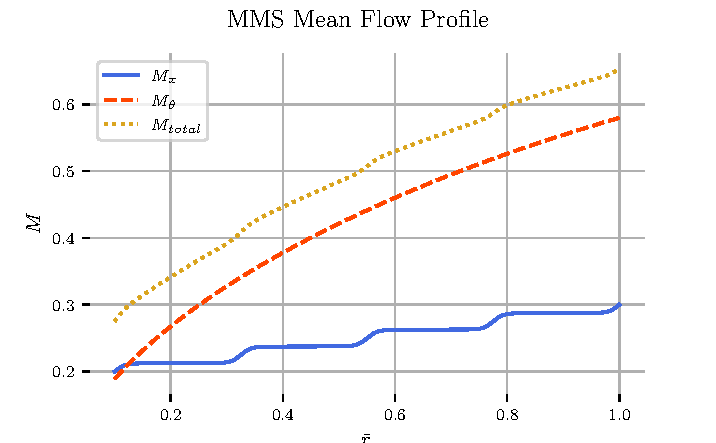
\includegraphics{/home/jeff-severino/SWIRL/CodeRun/03-plotReport/tex-outputs/MMS_mean_flow_profile.pdf}
    \caption{The manufactured mean flow test case using a summation of Tangents for $A$ and $M_x$}
    \label{fig:1}
\end{figure}

\begin{figure}[!]
    \centering
    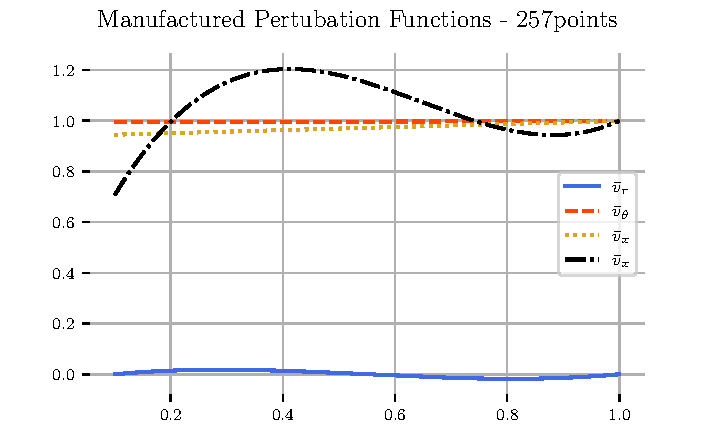
\includegraphics{/home/jeff-severino/SWIRL/CodeRun/03-plotReport/tex-outputs/MMS_perturbation_variables.pdf}
    \caption{The manufactured perturbation functions ,$v_r$, $v_x$, $v_{\theta}$, $p$}
    \label{fig:1a}
\end{figure}

\begin{figure}[!]
    \centering
    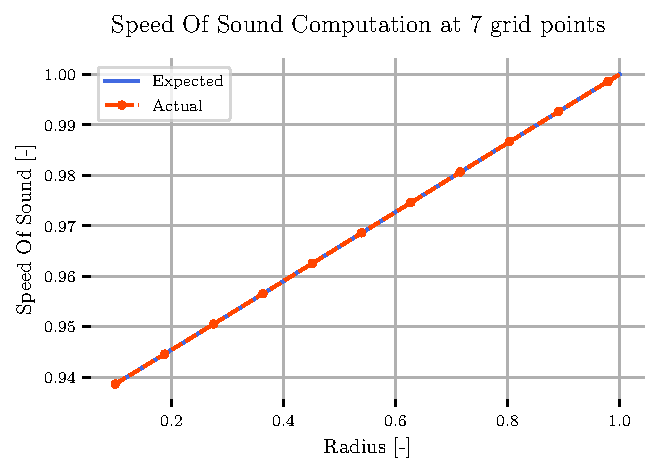
\includegraphics{/home/jeff-severino/SWIRL/CodeRun/03-plotReport/tex-outputs/SpeedOfSoundComparison1.pdf}
    \caption{Expected L2 Norm vs the calculated and the line of best fit of 
    the calculated L2}
    \label{fig:2}
\end{figure}

The standard form of a logarithmic function was used plot a line of constant
slope of two as it was superimposed on the approximated L2 norm ,$\hat{epsilon}$. 
A line of best fit was determined using a curve fitting techique and the y 
intercept was approximated to be the same at the approximated L2 data but the slope
found is slightly higher than expected. 


\begin{figure}[!]
    \centering
    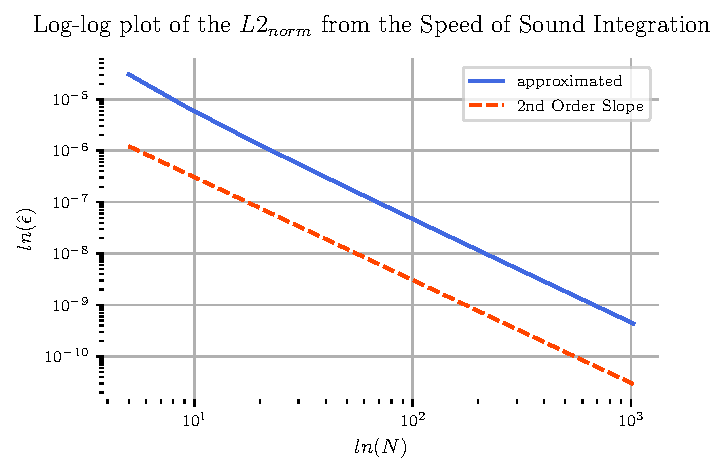
\includegraphics{/home/jeff-severino/SWIRL/CodeRun/03-plotReport/tex-outputs/SND_L2.pdf}
    \caption{}
    \label{fig:4}
\end{figure}


\begin{figure}[!]
    \centering
    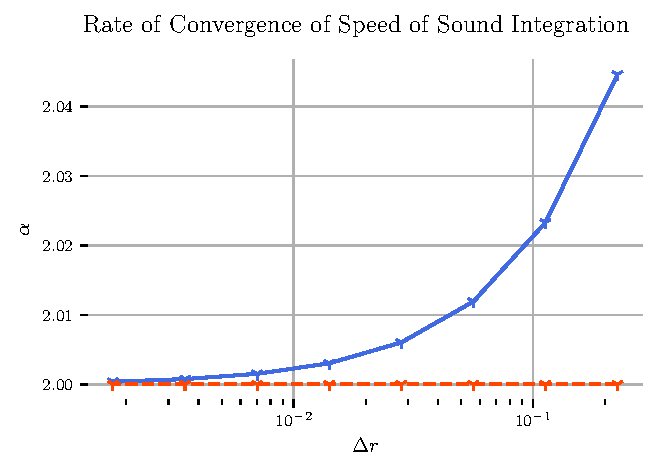
\includegraphics{/home/jeff-severino/SWIRL/CodeRun/03-plotReport/tex-outputs/SND_ROC.pdf}
    \caption{}
    \label{fig:5}
\end{figure}

\section{Planned Research}
If these plots for the MMS are sufficient for the Speed of Sound then the same 
graphs will also be shown for each source term. 


\end{document}


